\chapter{Implementation overview}

\section{Architecture and design schemes}

\subsection{Software architecture}

The application provides the drawing surface and callback functions for Moai SDK, to which it is connected via the AKU interface.
Moai Qt Host is implemented with Qt so it uses Qt libraries in implementation. The main architecture of Moai Qt Host is shown in figure \ref{fig:modules}

\begin{figure}[h]
	\begin{center}
	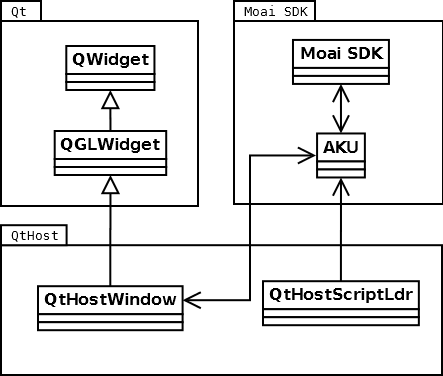
\includegraphics[scale=0.6]{images/moai_qt_host_modules.png}
	\caption{Moai Qt Host modules\label{fig:modules}}
	\end{center}
\end{figure}

\subsection{Hardware architecture}

There is no hardware architecture connected to the application.

\subsection{Database architecture}

Moai SDK does not use a database.

\subsection{Network architecture}

No network architecture is needed in the current version.

\section{Modules}

The design ideology of Moai Qt Host is modular, so new modules can be easily added. Currently there are only two modules. See figure~\ref{fig:modules}. QtHostWindow module provides drawing surface for Moai and handles input events. QtHostScriptLdr module reads in given Lua scripts. Initialization of Moai and host modules are done in the main-function of the application.


\section{Datastructures}

Not specified.

\section{Database}

No database is used.

\section{User interface}

There is no user inferface besides the main window frame.

\section{Printing}

There is no printing functionality.

\section{Errors and recovery}

All errors are handled in-program.

\section{Security and protection}

Not specified.
